                                               %%%%%%%%%%%%%%%%%%%%%%%%%%%%%%%%%%%%%%%%%%%%%%%%%%%%%%%%%%%%%%%%%%%%%%%%%%%%%%%
%%% SWEAVE
       % Ihaka, R. (2009). Customizing Sweave 
%%%%%%%%%%%%%%%%%%%%%%%%%%%%%%%%%%%%%%%%%%%%%%%%%%%%%%%%%%%%%%%%%%%%%%%%%%%%%%%
%%% CUSTOMIZING SWEAVE 
%%% from: Ihaka, R. (2009). Customizing Sweave to Produce Better Looking LATEX Output
\DefineVerbatimEnvironment{Sinput}{Verbatim}{fontsize=\footnotesize, formatcom=\color{codecolor}, xleftmargin=2em}
\DefineVerbatimEnvironment{Soutput}{Verbatim}{fontsize=\footnotesize, xleftmargin=2em, formatcom=\color{codecolor}} 
\DefineVerbatimEnvironment{Scode}{Verbatim}{fontsize=\footnotesize, xleftmargin=2em, formatcom=\color{codecolor}}

\renewenvironment{Schunk}{\vspace{10pt}}{\vspace{8pt}}   
%%%%%%%%%%%%%%%%%%%%%%%%%%%%%%%%%%%%%%%%%%%%%%%%%%%%%%%%%%%%%%%%%%%%%%%%%%%%%%%
%%%%%%%%%%%%%%%%%%%%%%%%%%%%%%%%%%%%%%%%%%%%%%%%%%%%%%%%%%%%%%%%%%%%%%%%%%%%%%%

\section{Stichprobenverteilung von Korrelationskoeffizienten}

Signifikanstests und Konfodenzintervalle für Korrelationskoeffizeinten werden mit Hilfe von Fisher's Z-Transformation berechnet (nichts zu verwechselen mit der z-Transormation). Sie hat folgende Form.

\begin{equation} \label{eq:fisher}
  f(\varrho)=0{,}5\ln\left(\frac{1+\varrho}{1-\varrho}\right)  
\end{equation}                                               

\begin{Schunk}
\begin{Sinput}
> fisher.z <- function(r){
   .5 * log((1+r) / (1-r))
 }
\end{Sinput}
\end{Schunk}

% \begin{equation}
% z_1=f(r)-\frac{z_{1-\alpha/2}}{\sqrt{n-3}} \leq\mu\leq f(r)+\frac{z_{1-\alpha/2}}{\sqrt{n-3}}=z_2     
% \end{equation}  

Warum ist dies nötig und was bewirkt sie? Um dies besser zu verstehen sollen Korrelationskoeffizienten aus unterschielichen Populationen simuliert werden.

\begin{Schunk}
\begin{Sinput}
> sim_pop <- function(r, n=1000){
   x1 <- rnorm(n)
   x3 <- rnorm(n)
   x2 <- r * x1 + sqrt(1 - r^2) * x3
   data.frame(x1, x2) 
 }
> mean(replicate(1000, cor(sim_pop(.5))[1,2]))
\end{Sinput}
\begin{Soutput}
[1] 0.4999013
\end{Soutput}
\end{Schunk}

Die Daten werden korrekt erstellt. Um einen Eindruck von der Stichprobenverteilung von Korrelationskoeffizeinten zu bekommen erzeigen wir eine Population und ziehen aus dieser wiederholt eine Stichprobe auf dessen Basis wir die Korrelation errechnen.

\begin{Schunk}
\begin{Sinput}
> sample_dist <- function(r, n, nrep){
   x <- sim_pop(r, 1e5)
   res <- rep(NA, nrep)
   for (i in 1:nrep){
     index <- sample(1:nrow(x), n)
     res[i] <- cor(x[index, 1], x[index, 2])  
   }
   res  
 }
\end{Sinput}
\end{Schunk}

\begin{Schunk}
\begin{Sinput}
> x <- sample_dist(0, 100, 1e3)
> hist(x, breaks=40, xlim=c(-.5,1))  
\end{Sinput}
\end{Schunk}
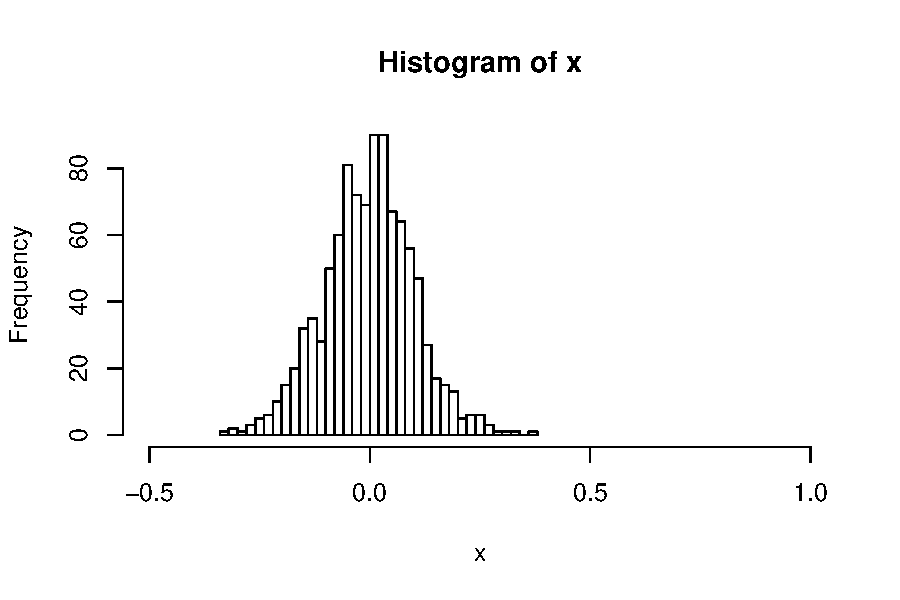
\includegraphics{sim_correlation-005}

Die Verteilung ist symmetrisch und errinnert an eine Gauß-Verteilung.
Die Wiederholen wir den Vorgang mit 

\begin{Schunk}
\begin{Sinput}
> x <- sample_dist(.7, 100, 1e3)
> hist(x, breaks=40, xlim=c(-.5,1))  
\end{Sinput}
\end{Schunk}
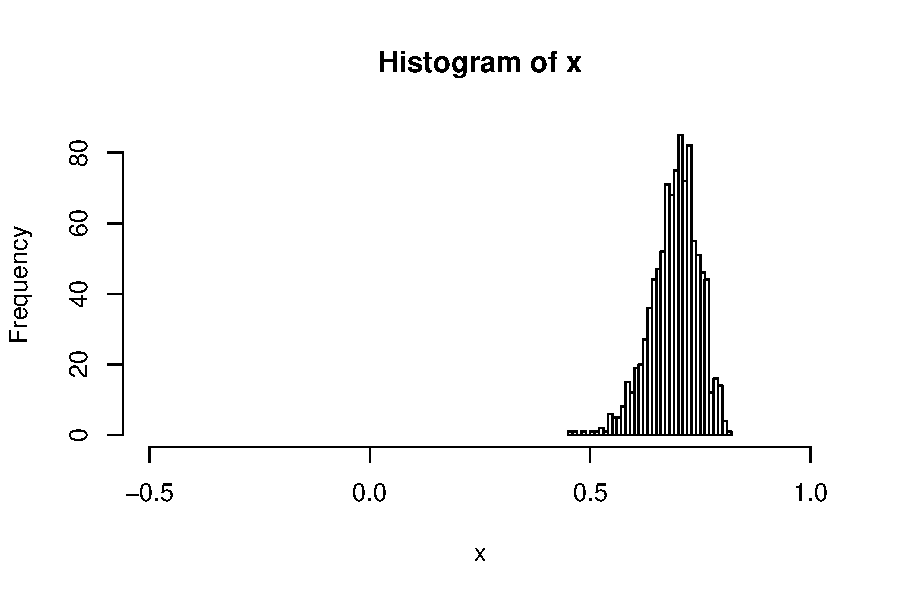
\includegraphics{sim_correlation-006}

Um dies besser zu verstehen simulieren wir Verteilungen für diverse $r$.
\begin{Schunk}
\begin{Sinput}
> r <- numeric()
> rpops <- seq(.3, .9, .2)
> for (i in seq_along(rs))
   r <- c(r, sample_dist(rpops[i], 100, 1000))
> rpop <- rep(rpops, each=1000)
> rz <- fisher.z(r)
> xr <- data.frame(rpop, r=r) 
> xz <- data.frame(rpop, r=rz) 
\end{Sinput}
\end{Schunk}

\begin{Schunk}
\begin{Sinput}
> library(ggplot2)
> g <- ggplot(xr, aes(x=r), ) +  geom_density() + 
             facet_grid(. ~ rpop)
> g
\end{Sinput}
\end{Schunk}
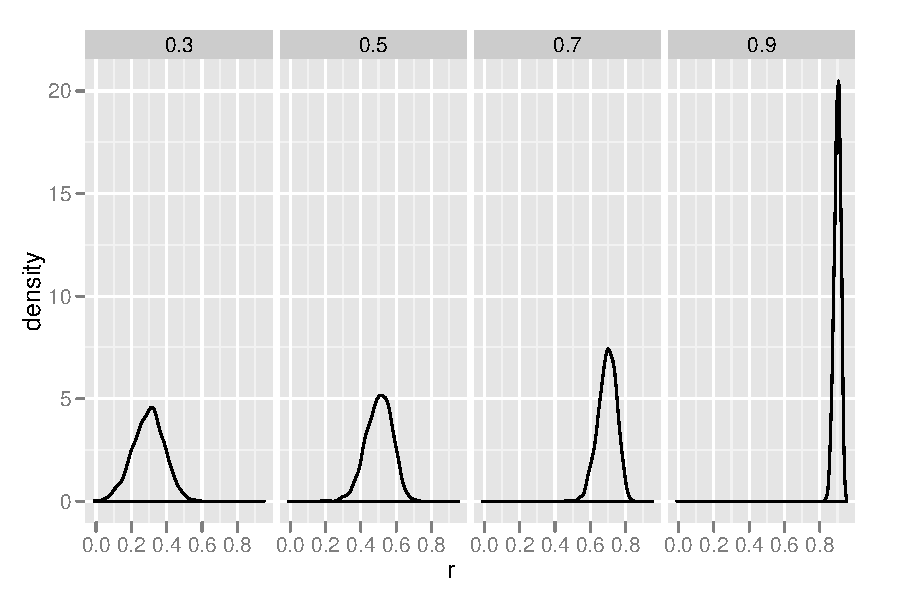
\includegraphics{sim_correlation-008}

\begin{Schunk}
\begin{Sinput}
> g %+% xz
\end{Sinput}
\end{Schunk}
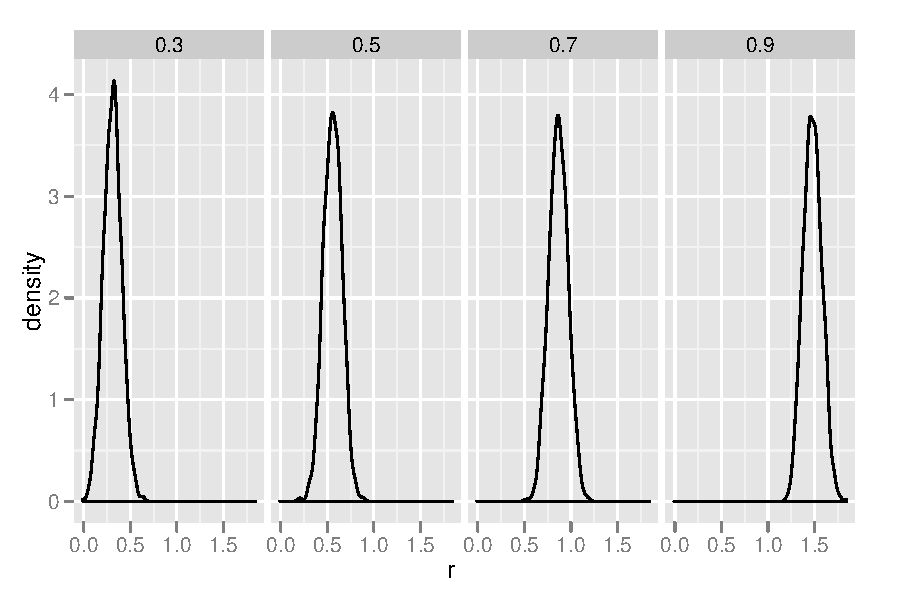
\includegraphics{sim_correlation-009}






